\documentclass[twoside,11pt]{article}

\usepackage{jmlr2e}
\usepackage{amsmath}
\usepackage[]{algorithm2e}


\ShortHeadings{Optimal spike-based signal representation on a neuromorphic chip}{Optimal spike-based signal representation on a neuromorphic chip}
\firstpageno{1}

\begin{document}


\title{Optimal spike-based signal representation\\on a neuromorphic chip}

\author{\name Julian B\"uchel \email jubueche@ethz.ch \\
       \addr Institute of Neuroinformatics\\
       University of Z\"urich, ETH Z\"urich \\
       Z\"urich, ZH, Switzerland}

\editor{}

\maketitle

\tableofcontents
\newpage

\begin{abstract}%   <- trailing '%' for backward compatibility of .sty file
This paper describes the mixtures-of-trees model, a probabilistic 
model for discrete multidimensional domains.  Mixtures-of-trees 
generalize the probabilistic trees of \citet{chow:68}
in a different and complementary direction to that of Bayesian networks.
We present efficient algorithms for learning mixtures-of-trees 
models in maximum likelihood and Bayesian frameworks. 
We also discuss additional efficiencies that can be
obtained when data are ``sparse,'' and we present data 
structures and algorithms that exploit such sparseness.
Experimental results demonstrate the performance of the 
model for both density estimation and classification. 
We also discuss the sense in which tree-based classifiers
perform an implicit form of feature selection, and demonstrate
a resulting insensitivity to irrelevant attributes.
\end{abstract}

\begin{keywords}
  Bayesian Networks, Mixture Models, Chow-Liu Trees
\end{keywords}

\section{Introduction}

- Why is it important to represent signals?
- What are desirable properties when representing a signal?
(fault tolerance (not only a few neurons contribute), cost efficiency, reconstruction error,
generalization, adaptation)
- Where could this be useful? 
-Machine learning (transform input to sparse high dimensional vectors
and use representation to eg learn, denoise, cluster etc)
- Neuro Agents who encounter signals of the same domain very often and want to represent
these signals with as few spikes as possible
- Links to general thesis that agents want to minimize free energy? Friston?

\section{Theory: Representing signals spike-by-spike}
\subsection{Introduction}
Is tight E/I-balance better than loose? What do the studies suggest? What do rodents or 
other animals do? What about rate encoding?
In the following we derive a learning rule that achieves a tight E/I-balance and 
minimizes reconstruction error and generates sparse spike trains.

We will show only the learning rules for the recurrent connections.

\subsection{Network dynamics}
%Define voltage equation(diff and explicit), rate equation, reconstructed x
%State assumptions such as fully connected, not respecting Dales law. Also state that these
%assumptions can be relaxed and reference to paper that achieves this

In this work, we assume that we have a population of $N$ neurons into which $N_x$ continous
signals are fed using a linear transformation $\mathbf{F}$. We furthermore assume that the population
of $N$ neurons is fully interconnected by a matrix $\mathbf{\Omega}$. It is thus beneficial to assume 
the computationally efficient Leaky Integrate-and-Fire (LIF) neuron model (cite LIF). 
The network dynamics can thus be written as

\begin{equation} \label{voltage_dynamic_diff}
    \dot{V}(t) = -\lambda V(t) + \mathbf{F^T}c(t) + \mathbf{\Omega} o(t) 
\end{equation}
%Where klein
Where $c(t)$ is the input signal at time $t$ and $o(t)$ the spike train of the population, also at
time $t$. By defining a filtered version of the input $c$ and the spike train $o$, we can integrate Equation \ref{voltage_dynamic_diff}
to
%! Not V(t+1)?!
\begin{equation} \label{voltage_dynamic_explicit}
    V(t) = \mathbf{F^T}x(t) + \mathbf{\Omega} r(t)
\end{equation}
where we define
\begin{equation} \label{rate_diff}
    \dot{r}(t) = -\lambda r(t) + o(t)
\end{equation}
and 
\begin{equation} \label{input_diff}
    \dot{x}(t) = -\lambda x(t) + c(t)
\end{equation}
For the simulations conducted in this thesis, uncorrelated inputs where used. These were generated
by simply convolving white noise with a gaussian filter of width $\sigma$. An example of a typical
input used throughout this thesis is presented in Figure \ref{fig:input}.

\begin{figure}[!htb]
    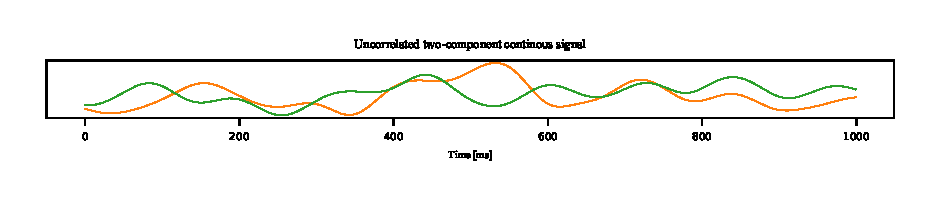
\includegraphics[width = \columnwidth, height=3cm]{figures/input.eps}
    \caption{Input $x$ of dimension $N_x = 2$ shown over a period of 1000 ms.}
    \label{fig:input}
\end{figure}

It should be noted that for the sake of mathematical simplicity, as well as ease of
transformation to a neuromorphic chip, this setup does not respect Dales law, as it
allows for neurons to be excitatory and inhibitory at the same time. However, (cite Brendel)
also derives learning rules that respect the more biologically plausible setup.

We furthermore assume a readout layer, or decoder, that reconstructs the input $x$ using
the rates exposed by the population. The reconstructed signal can be defined as

\begin{equation} \label{reconstructed_x_explicit}
    \mathbf{\hat{x}} = \mathbf{Dr}
\end{equation} 
where the decoder $\mathbf{D}$ is a matrix of size ($N_x$,$N$), $\mathbf{r}$ is a matrix of shape
($N$,$N_\textnormal{time}$) and $\mathbf{x}$ is a matrix of shape ($N_x$,$N_\textnormal{time}$).

\subsection{The optimal decoder}

Keeping in mind the goals that we are following, namely low reconstruction error, low firing
rates and even distribution across neurons, we can define the following loss function, balancing
low reconstruction error with sparse (\textit{l1}-cost) and dense (\textit{l2}-cost) spike trains.

\begin{equation} \label{loss_function_optimal_decoder}
    L^* = \min_{o} \|\mathbf{x} - \mathbf{Dr}\| ^2_2 + \mu \|\mathbf{r}\|_2^2 + \nu \|\mathbf{r}\|_1
\end{equation}

Because of Equation \ref{rate_diff}, one can see that enforcing \textit{l2}-sparsity allows for
dense population codes (since it keeps the rates genereally low, but does not enforce 0 values). 
In contrast, \textit{l1}-sparsity encourages 0 values in the rates, which correponds to sparse spike trains (cite spars.).
This loss function gives us an explicit formula for the optimal decoder that is achievable by the network.
By taking the derivative of Equation \ref{loss_function_optimal_decoder} with respect to $\mathbf{D}$ and setting it to \textbf{0}, we get

\begin{equation} \label{optimal_decoder_no_lagrangian}
    \mathbf{D}^* = \mathbf{xr^T}(\mathbf{rr^T})^{-1}
\end{equation}


\subsection{Optimal network connectivity}
%First derive the optimal connectivity assuming we have the optimal decoder. p. 7-8
%Mention the derivation involving one spike per time as this imposes a limit to our later work.
%Derive optimal network connectivity
Following (cite Brendel), we will now discuss how to optimize the network topology.
In particular the synaptic weights and the thresholds
under the assumption that the decoder is fixed. Note that letters such as
$r$ are not bold and thus stand for a vector in time, $r(t)$, which is abbreviated for clarity.
The main idea (cite Learning optimal spike-based representations) behind the
following derivation is that a neuron in the population should only spike if it
contributes to the reduction of the loss function.
This means that

\begin{equation} \label{loss_smaller}
  \textit{L(neuron n spikes)} < \textit{L(neuron n does not spike)}
\end{equation}

Using Equation \ref{loss_function_optimal_decoder}, $\textit{L(neuron n spikes)}$ can be
written as

\begin{equation} \label{neuron_n_spiked_loss}
  \textit{L(neuron n spikes)}=\|c-Dr-D_n \|_2^2+\mu\|r+e_n\|^2_2+\nu\|r+e_n\|_1
\end{equation}
where $e_n$ is the unit vector with $(e_n)_j = 1$ if $j=n$ and 0 else.

We observe that
\begin{equation} \label{rate_plus_unit_l2}
  \|r+e_n\|^2_2 = (\sum_{i,i \neq n}r_i) + (r_n+1)^2 = \|r\|^2_2 + 2r_n + 1
\end{equation}
and
\begin{equation} \label{rate_plus_unit_l1}
  \nu \|r + e_n\|_1 = \nu (\sum_{i,i\neq n}|r_i|) + \nu |r_n+1| =^* \nu (\sum_{i,i\neq n}|r_i|) + \nu |r_n| +\nu = \nu \|r\|_1 + \nu  
\end{equation}
where * holds because $\forall t \; r(t) \geq 0$.
Using Equations \ref{rate_plus_unit_l2} and \ref{rate_plus_unit_l1} we can rewrite Equation
\ref{loss_smaller} to

\begin{equation} \label{network_dynamics}
  D_n^Tc - D_n^TDr - \mu r_n > \frac{1}{2} (\| D_n\|^2_2 + \mu + \nu) 
\end{equation}

This condition enforces that neuron $n$ only fires a spike, when it contributes
to the reduction of the global error. We observe,
under the assumption that the decoder is fixed, that the r.h.s. is constant and the l.h.s. is 
time-dependent, as it depends on $c$ and $r$.
It is therefore natural to denote the voltage of neuron $n$ as

\begin{equation} \label{voltage_via_dynamics}
  V_n(t) = D_n^Tc(t) - D_n^TDr(t) - \mu r_n 
\end{equation}
and the threshold of the $n$-th neuron as
\begin{equation} \label{threshold_via_dynamics}
  T_n = \frac{1}{2} (\| D_n\|^2_2 + \mu + \nu)
\end{equation}

using the differential equations \ref{input_diff} and \ref{rate_diff}, as well as Equation \ref{voltage_dynamic_diff}
we rewrite Equation \ref{voltage_via_dynamics} to

\begin{equation} \label{voltage_diff_via_dynamics}
  V(t) = \mathbf{F^T}x(t) + \mathbf{\Omega} o(t)
\end{equation}
where we substituted $\mathbf{F} = \mathbf{D}$ and $\mathbf{\Omega} = -\mathbf{D^TD} - \mu \mathbf{I} = -\mathbf{F^TF} - \mu \mathbf{I}$, which are the optimal feed-forward and
recurrent weights in the network, with respect to the decoder.

We also note that since $\mathbf{\Omega} = -\mathbf{D^TD} - \mu \mathbf{I}$, we have $T = \frac{1}{2}(\textnormal{diag}(\mathbf{\Omega}) + \nu)$.
This way the error dictates the produced spike train, hence \emph{error-driven coding}.

Since neurons have a "fixed" threshold, Equation \ref{threshold_via_dynamics} can be seen
as a constraint on the decoder length for a neuron by simply rewriting it to

\begin{equation} \label{threshold_rewritten}
  \|D_n\|_2^2 = 2T_n - \mu - \nu
\end{equation} 


\subsection{Learning optimal recurrent connectivity}
%Show, mathematically, that a balanced network ensures low recontruction error, assuming
%the voltage represents the error
%From the previous subsection we derive the recurrent weight learning rule, based on the fact 
%that a balanced network suffices.
We have seen from the previous section that the voltage encodes the global loss and
that a neuron fires a spike only to reduce the reconstruction error.
This corresponds to the hypothesis that a tightly balanced network exhibits a low reconstruction
error, as discussed in section (ref section).
This however corresponds to the state where $\mathbf{x} - \mathbf{\hat{x}} \approx 0$.
We observe that the neuron has only access to the linearly transformed version: $F_n^T\mathbf{x} - F_n^TD\mathbf{r}$. 
However, this value should also be close to zero, as it reflects part of the reconstruction error.

\begin{equation} \label{balanced_voltage}
  \begin{split}
    \epsilon_n &= F^T_n\mathbf{x}-F^T_n\mathbf{\hat{x}} \\
    &= F_n^T - F^T_n\mathbf{Dr} \\
    &\approx 0
  \end{split}
\end{equation}

We furthermore observe, using the optimal feed-forward and recurrent connections, that Equation
\ref{balanced_voltage} corresponds to the network dynamics obtained in Equation \ref{voltage_dynamic_explicit}.
We can conclude that the signal is represented optimally if $\Omega_n = -F^T_n\mathbf{D}$, $\epsilon_n = V_n \approx 0$ and
$\mathbf{D} = \mathbf{D}^*$.
From this, we are now able to derive a learning rule for the recurrent weights, that will yield
the optimal solution.

In order to achieve a balanced network, it is desirable that over the long run, the
membrane voltages before and after a presynaptic spike cancel each other:

\begin{equation} \label{loss_voltage_before_after}
  L(t_j) = \| \frac{1}{2} (V^{\textnormal{before}}(t_j)+V^{\textnormal{after}}(t_j)) \| ^2_2
\end{equation}
Note that we add the two voltages since we assume that the voltage jumps from the positive to the
negative domain.
After the arrival of a presynaptic spike at time $t_j$ of neuron with index $k(j)$, the voltages are changed and the following relation is formed:

\begin{equation} \label{relation_voltage_before_after}
  V^{\textnormal{after}} = V^{\textnormal{before}} + \mathbf{\Omega} e_{k(j)}
\end{equation}

where $e_{k(j)}$ is the unit vector with 1 at the position of the neuron that spiked.
Using this relation we can rewrite the Equation \ref{relation_voltage_before_after} to

\begin{equation*} 
  L = \|V^{\textnormal{before}} + \frac{1}{2}\mathbf{\Omega} e_{k(j)}\|^2_2
\end{equation*}

this term has the derivative, with respect to $\Omega_{n,k}$:

\begin{equation}
    \Delta \Omega_{n,k} = -2V^{\textnormal{before}}_n - \Omega_{n,k}
\end{equation}

if neuron $k$ spiked. The connection $\Omega_{n,k}$ is the connection from the spiking, presynaptic neuron with index $k$ to the $n$-th neuron.

If we induce a small \textit{l2}-cost on the rates, $\mathbf{\Omega}$ should ideally converge towards $-\mathbf{F^TD} - \mu \mathbf{I}$. This causes a minor change in the learning rule for the recurrent weights:
\begin{equation} \label{updated_recurrent_learning_rule}
    \Delta \Omega_{n,k} = -2(V^{\textnormal{before}}_n + \mu r_n) - \Omega_{n,k} - \mu \delta_{n,k}
\end{equation}

where $\delta_{n,k}$ is $[e_n]_j$ and therefore 1 if $n =j$.


\subsection{Simulation and results}
%State the pseudo code when using only recurrent connections.
%Show figures of the weight convergence, the error convergence, variance of membrane potential
%mean firing rate and actual decoding that is happening.
Learning the feed-forward connections happens on a much slower timescale and thus requires
far more training iterations. Since the DYNAPS operates on a much slower, biologically
more plausible timescale (cite DYNAPS), training takes orders of magnitude longer. We therefore decided to omit
learning the feed-forward weights and keep them constant after an initial random initialisation.
The pseudo code presented below was adapted from (cite Brendel) and shows the learning procedure.

\vspace{1cm}
\IncMargin{1em}
\begin{algorithm}[H]
  \DontPrintSemicolon
  \label{algorithm_simulation}
  \KwIn{Number of training iterations $N_\textnormal{iter}$}
  \KwOut{Learned recurrent matrix $\mathbf{\Omega}$}
  \BlankLine
  $T \leftarrow \textnormal{N}_\textnormal{iter} \cdot \textnormal{N}_{\textnormal{time}}$\;
  $\textit{thresh} \leftarrow 0.5$ \;
  \For{$i \leftarrow 0$ \KwTo $T$}{
    \If(\tcp*[h]{Generate new input}){$i \; \textnormal{mod} \; \textnormal{N}_{\textnormal{time}} = 0$}{
      $Input \leftarrow \mathcal{N}(\mathbf{0}, \mathbf{I})$ \;
      $Input \leftarrow A \cdot (Input \ast w)$ \;
    } 
    $t \leftarrow (i \; \textnormal{mod} \; \textnormal{N}_{\textnormal{time}})+1$ \;
    $V_t \leftarrow (1-\lambda dt) \cdot V_{t-1}+dt \cdot \mathbf{F^T}\textnormal{Input}_t+\mathbf{\Omega} o_{t-1}+\epsilon \cdot \mathcal{N}(0,1) $ \;
    $x_t \leftarrow (1-\lambda dt)\cdot x_{t-1}+dt\cdot  \textnormal{Input}_t$ \;

    $(\textnormal{max},k) \leftarrow \textnormal{arg max}(V_t - \textit{thresh}-0.01 \cdot \mathcal{N}(0,1))$ \;
    \eIf(\tcp*[h]{Neuron k spiked}){$\textnormal{max} \geq 0$}{
      $\Omega_k \leftarrow \Omega_k-\epsilon_\Omega \cdot (\beta \cdot (V_t + \mu \cdot r_{t-1})+\Omega_k+\mu \cdot I_k)$ \;
      $r_t \leftarrow r_{t-1} + I_k$ \;
    }
    {
      $r_t \leftarrow r_{t-1}$
    }
    $r_t \leftarrow (1 - \lambda dt) \cdot r_t$ \;
  }
  \caption{Algorithm describing the learning procedure without learning the feed-forward weights.
  The used prameters can be found in the Appendix.  $\Omega_k$ and $I_k$ reference the
  $k$-th column of the respective matrix and $\ast$ is the convolution operator.}
\end{algorithm}
\DecMargin{1em}
\vspace{1cm}

Given the randomly initialized feed-forward matrix $\mathbf{F}$, we can measure the distance
between $\mathbf{\Omega}$ and $\mathbf{\Omega}^* = \mathbf{-F^TF}$, even if $\mathbf{F}$ is not learned.
As expected, the recurrent connection matrix converges towards the
optimal connectivity (Figure \ref{fig:convergence}(i)).
Initially, the network is in an unbalanced state and the
voltage predominantly reflects the transformed input.
After learning the recurrent weights, incoming excitatory signals are matched by
recurrent inhibition to keep the network in a tightly balanced state. This effect can be
observed in Figure \ref{fig:convergence}(ii) where we show the variance of the
membrane potential over time. By converging towards the optimal recurrent connection
and keeping the network in a tight balance, we fulfill the conditions necessary
for representing the signal optimally. The result of this can be seen
in Figure \ref{fig:convergence}(iii), where
the reconstruction error converges towards the discretization limit imposed by the
neurons. Since the learning rule keeps the network in a tight balance, no spike is fired
unnecessarily. Each spike, following Equation \ref{loss_smaller}, contributes
to reducing the global reconstruction error. This way, the resulting spike train sparsifies,
which can be observed in Figure \ref{fig:convergence}(iv). \\

\begin{figure}[!htb]
  \includegraphics[width = \columnwidth, height=12cm]{figures/convergence.eps}
  %! Correct caption please
  \caption{Multiple figures in here: (i) Convergence of optimal weights
  (ii) Convergence of membrane variance (iii) Convergence of error (iv) Convergence
  of firing rate}
  \label{fig:convergence}
\end{figure}
\newpage

To see the effect of learning, we trained the network for 140
iterations on different signals from the same domain. After the training process, we
computed the optimal decoder for the network using $\mathbf{\Omega}_{\textnormal{initial}}$ and
for the network using $\mathbf{\Omega}_{\textnormal{post learning}}$. We then generated a
new input $x$, which was then fed into the networks.
Using the decoder previously computed, we then reconstructed the signal and
compared the reconstruction quality. Figure \ref{fig:reconstruction} shows the different
reconstructions and spike trains of each network. As expected, results using
$\mathbf{\Omega}_{\textnormal{initial}}$ produced a poor reconstruction
compared to the network using $\mathbf{\Omega}_{\textnormal{post learning}}$.
It is also visible from the spike trains that the voltage initially
only represents the transformed input and later becomes more distributed across
the population.


\begin{figure}[!htb]
  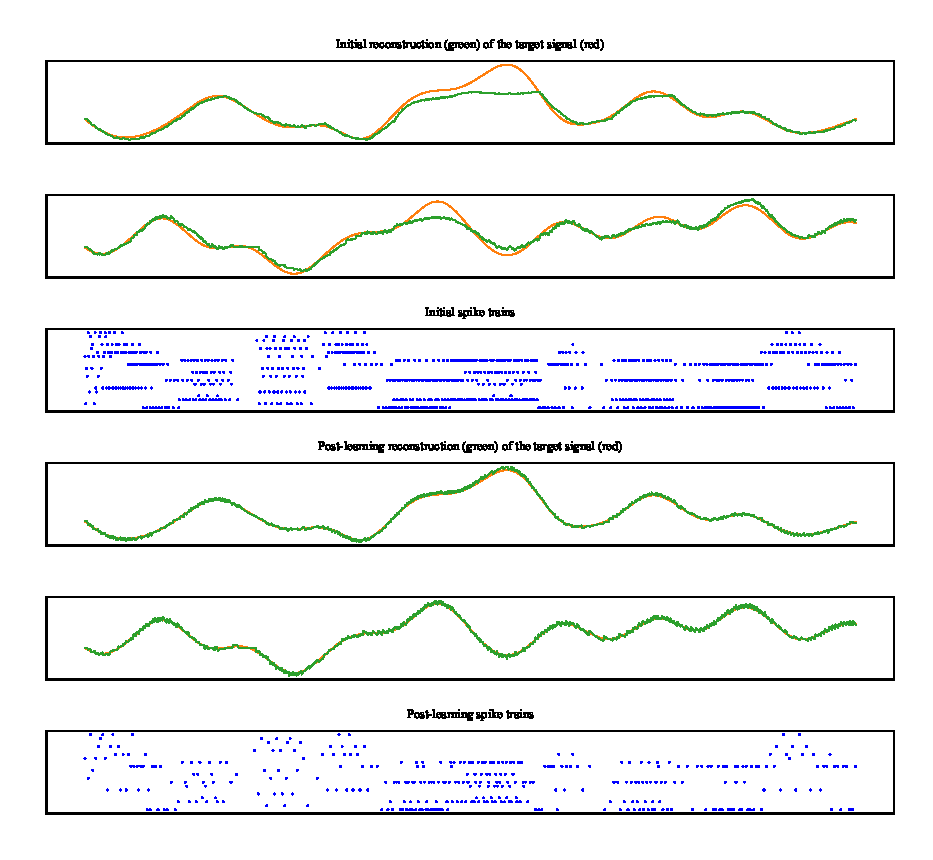
\includegraphics[width = \columnwidth, height=14cm]{figures/reconstruction.eps}
  \caption{Multiple figures in here: (i) Convergence of optimal weights
  (ii) Convergence of membrane variance (iii) Convergence of error (iv) Convergence
  of firing rate}
  %! Correct caption please
  \label{fig:reconstruction}
\end{figure}
\newpage

\subsection{Limitations of the theory} \label{sec:limitations}
%Discrete weights, taking the neuron with the maximum voltage above threshold to compute
%the rate vectors and do the updates. (Need to check if fails when using all neuons)
%Provide figures showing: Number of bins vs. recon error after 14000 iterations.
%Another figure showing two figures when using all neurons in the update.
Unfortunately, the theory proposed by (cite Brendel) has some limitations: \\
1) Discretization of the weights causes unsuccessful learning of the recurrent matrix and therefore
does not lead to improved sparsity and reconstruction error. \\
2) Updating the rate, as well as all outgoing connections of \emph{all} neurons that spiked,
results in no improvement of the mean firing rate and the reconstruction error. \\

In terms of biological plausibility, the first issue is far more severe than the second one. It is well
known that, although microcircuits can show dense connections (cite nature2016), the weight resolution
in the brain is limited to only a few bits (need citation). In this theory, tight balance of the input
currents is of crucial importance. When discretizing the weights, this balance can no longer
be achieved and therefore the network seems to fire uncontrollably, as can be seen in Figure
\ref{fig:discrete_spike_trains}. Naturally, this uncontrolled firing causes high reconstruction
error and the learned matrix becomes irrelevant (Figure \ref{fig:convergence_ua_discrete}).

\begin{figure}[!htb]
  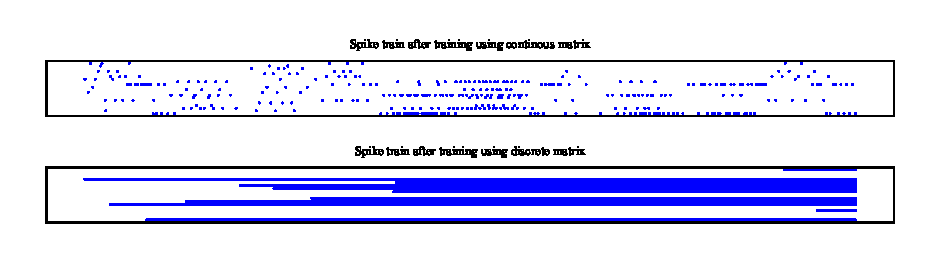
\includegraphics[width = \columnwidth, height=4cm]{figures/spike_train_cont_vs_disc.eps}
  \caption{The spike train after training using continous weights (top), exhibits a usable,
  distributed pattern, while the learned, discretized weight matrix (bottom) shows a subset
  of neurons firing at a high frequency.}
  %! Correct caption please
  \label{fig:discrete_spike_trains}
\end{figure}

Assuming a continous timescale, there can not be an instance in time, where two neurons fire simultaneously.
However, in the simulations, as well as on the DYNAPS (cite DYNAPS), time is discretized and therefore
the event that two neurons fire at the same time \emph{can} happen.
When adapting Equation \ref{relation_voltage_before_after} to account for this possibility and rewriting
the update rule accordingly, we found that the recurrent weights were still learned. Furthermore, the
varation in the membrane potential also decreased, which is explained by the fact that we are still
minimizing the loss in Equation \ref{loss_voltage_before_after}.
However, the derivation of the optimal network connectivity
in Equation \ref{network_dynamics} falsely assumes only one spike per time.
\newpage

\begin{figure}[!htb]
  \includegraphics[width = \columnwidth, height=16cm]{figures/convergence_d_vs_ua.eps}
  \caption{Convergence of different properties when learning with discrete weights (orange)
  and performing the updates with respect to all spiking neurons (green).
  It should be noted that the mean firing rate is really high compared to the successful learning (see
  Figure \ref{fig:convergence}).}
  %! Correct caption please
  \label{fig:convergence_ua_discrete}
\end{figure}

\newpage

\section{Hardware: The DYNAPS chip} \label{sec:DYNAPS}

\section{Learning optimal spike-based signal representations on the DYNAPS}
\subsection{Setup: Learning in-the-loop}
%This section describes the learning procedure using a diagram. Should be one page max.
Although spike-timing dependent plasticity is implemented on-chip (citation), this learning
algorithm requires an in-the-loop setup. The reason for this was already pointed out in
section \ref{sec:limitations}: Discretizing the weights in the simulation
makes learning impossible, even with a relatively high number of bins. This is why
we have to keep a continous off-chip version of the recurrent matrix during learning.
In this setup, we repeatedly present a signal to
the chip, record the emitted spikes and perform the matrix update off-chip. The updated
matrix is then rescaled, discretized and loaded onto the chip and the process starts
all over again (see Figure \ref{fig:in-the-loop}). For a more detailed description of the
program see section \ref{sec:pseudo-code}.

\begin{center}
  \begin{figure}[!htb]
    \includegraphics[width = \columnwidth, height=7cm]{figures/in-the-loop.png}
    %! Correct caption please
    \caption{The feed-forward connections $\mathbf{F^TM}$ (derived in section \ref{sec:spiking-input}) are initially discretized to $\mathbb{Z}$
    and loaded onto the chip. The following four steps are executed repeatedly
    for a fixed number of iterations: A new signal is generated and stored in the
    FPGA memory, the recurrent weights $\mathbf{\Omega}$ are updated, discretized
    to $\mathbb{Z}$ and loaded onto the chip, the DYNAPS runs on the spiking input
     and finally $\Delta \mathbf{\Omega}$ is computed using the spike trains
    $\mathbf{O}^{\textnormal{DYNAPS}}$ recorded from the DYNAPS.}
    \label{fig:in-the-loop}
  \end{figure}
\end{center}

Since this setup utilizes the DYNAPS, which operates on a biologically plausible timescale,
this learning process takes orders of magnitudes longer than the off-chip simulation.

\newpage

\subsection{Aligning on- and off chip network dynamics}
\subsubsection{Network with spiking input} \label{sec:spiking-input}
%This section should describe how the continous input is converted to UP and DWN channels
%as well as the reconstruction using matrix M.
%We should also show that we can initially transform the input signal from the spike domain
%back to the continous domain, and then apply the transformation. But to match the DYNAPS, 
%we need a matrix with weights that takes care of this integration and transformation
%in the same time. In other words, we need to show that the matrix FtM*I provides the same
%functionality as Ftx\_hat where x\_hat is the reconstructed signal.
Information in the brain is processed in the analog and digital domain. Spikes, emitted from pre-synaptic
neurons, cause a change in the membrane potential of synapses leading to the emission of different
neurotransmitters. Inputs to the brain are converted to spikes using different nerve cells, such as the
photoreceptors in the retina. The DYNAPS also receives input in the form of spikes, which raises the question
on how to convert a continous signal to spikes. One simple approach called Delta Modulation (citationHere),
converts a 1D-signal to two channels, namely the UP and DOWN channel. The spikes emitted in the respective
channels depend on the magnitude and direction of the current signal slope. Figure \ref{fig:delta_modulated_input}
illustrates the spikes of a 1D-signal using 0.05 as a spiking threshold in both directions.


\begin{figure}[!htb]
  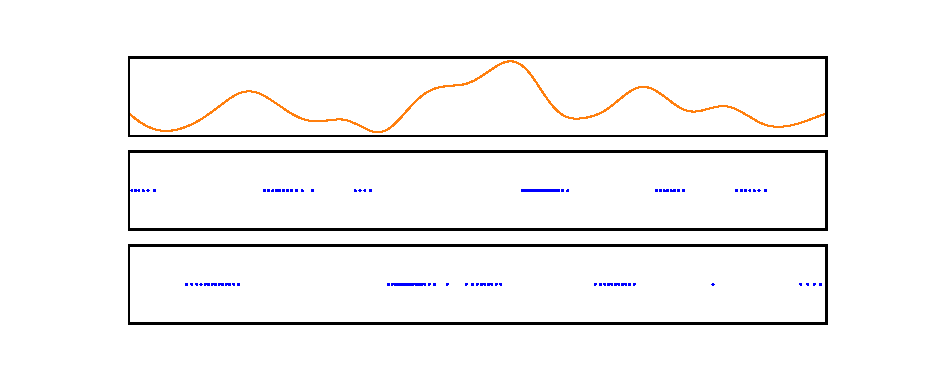
\includegraphics[width = \columnwidth, height=4cm]{figures/delta_modulated_input.eps}
  \caption{The signal (top) is split into two channels, representing the (upward) downward
  magnitude of the signal in the number of spikes.}
  %! Correct caption please
  \label{fig:delta_modulated_input}
\end{figure}

Going back to the simulation, one can see that the input to the network is 

\begin{equation}
  \textnormal{Input} = \mathbf{F^T}x
\end{equation}
where $\mathbf{F}$ is a matrix of size ($N_x$,$N$). By integrating the spikes using

\begin{equation} \label{recon_input}
  \hat{x}_t = (1-\lambda)\hat{x}_{t-1} + \nu(o^{up}_t - o^{down}_t)
\end{equation}
one can reconstruct a discretized version of the original signal $\hat{x}$ using appropriate values
for $\lambda$ and $\nu$. Using

\[M = \begin{bmatrix}
  1 & -1 & 0 & 0 \\ 
  0 & 0 & 1 & -1
  \end{bmatrix}
\]

the general form of Equation \ref{recon_input} becomes

\begin{equation}
  \hat{x}_t = (1-\lambda)\hat{x}_{t-1} + \nu Mo_t
\end{equation}

In order to match the simulation with the DYNAPS, one could simply integrate the spikes and transform
the reconstructed signal to get an approximation of the input using

\begin{equation}
  \textnormal{Input} = \mathbf{F}^T \hat{x} = \mathbf{F}^T((1-\lambda)\hat{x}_{t-1} + Mo_{t-1})
\end{equation}

This however does not match the setup on the DYNAPS since the input is first transformed using $M$, then
integrated and then again transformed using $F$. Contrary, the synapses on the DYNAPS first integrate the
incoming spikes and then transform the integrated value using the weights. We therefore introduce a new variable
$I_t$ that symbolizes the current at time $t$ of the synapses. $I_t$ performs a simple integration of the input:

\begin{equation*}
  I_t = (1-\lambda)I_{t-1} + \nu o_t
\end{equation*}

By expanding the recursive definition for $k$ time steps and assuming that $(1-\lambda)^k$ becomes
negligibly small for some $k$ we get that

\begin{equation*}
  \begin{split}
      F^T \hat{x}_t & = F^T((1-\lambda) \hat{x}_{t-1} + \nu Mo_t) \\
      & = F^T((1-\lambda) \;... \;(1-\lambda)( (1-\lambda) \hat{x}_{t-k} + \nu Mo_{t-k+1}) + \nu Mo_{t-k+2} + ... + \nu Mo_t) \\
      & \approx F^T((1-\lambda)^{k-1} \nu Mo_{t-k+1} + (1-\lambda)^{k-2} \nu Mo_{t-k+2} + ... + (1-\lambda)^{0} \nu Mo_{t}) \\
      & = (1-\lambda)^{k-1} \nu F^TMo_{t-k+1} + (1-\lambda)^{k-2} \nu F^TMo_{t-k+2} + ... + (1-\lambda)^0 \nu F^TMo_t
  \end{split}
  \end{equation*}

is equal to

\begin{equation*}
  \begin{split}
      F^T M I_t & = F^T M ((1-\lambda) I_{t-1} + \nu o_t) \\
      & = F^T M((1-\lambda) ... (1-\lambda)( (1-\lambda) I_{t-k} + \nu o_{t-k+1}) + \nu o_{t-k+2} + ... + \nu o_t) \\
      & \approx F^T M((1-\lambda)^{k-1}\nu o_{t-k+1} + (1-\lambda)^{k-2}\nu o_{t-k+2} + ... + (1-\lambda)^{0}\nu o_{t}) \\
      & = (1-\lambda)^{k-1}\nu F^TMo_{t-k+1} + (1-\lambda)^{k-2}\nu F^TMo_{t-k+2} + ... + (1-\lambda)^0 \nu F^TMo_t
  \end{split}
\end{equation*}

We have shown that having real input transformed using a feed-forward matrix $F$ is approximately the same
as integrating a spike train $o_t$ and transforming it using the new matrix $F^TM$. This
scheme was successfully verified in the simulation. Figure \ref{fig:spiking_vs_continous} compares the reconstruction error over time
between the continous-input network and the spiking-input network.
Since the DYNAPS is doing the integration implicitly, we can simply set the feed-forward
connections to a discretized version of $F^TM$ and feed the delta modulated input to the chip. Unfortunately,
input precision is lost due to the discretization limit imposed by the spikes and more severly by the
weight resolution on the DYNAPS, which will be covered in another section.

\begin{figure}[!htb]
  \includegraphics[width = \columnwidth, height=4cm]{figures/error_convergence_use_spiking_vs_normal.eps}
  \caption{While the error convergence of the spiking-input and continous-input network matches,
  the error of the spiking-input network is increased by roughly a factor of 10, due to the
  loss of precision imposed by the spikes (note the green scale).}
  %! Correct caption please
  \label{fig:spiking_vs_continous}
\end{figure}

\newpage

\subsubsection{The weights on-chip}
%-This section explains the limitation of the DYNAPS with the synapses (fan-in 64,fan-out 4k, p.7 sec.4,DYNAPS_paper)
%-It explains that precision is lost due to the small fan in. It also
%explains how the weights are rescaled so that the relative size of Omega is kept using min max binning.
%- It then explains what possible ways are of dealing with too many neurons in fan-in and how to downgrade
%the neurons and what issues can occur when not doing it right, like for example 700/740 used,
%750/740 used -> too many -> scale down evenly -> 650/740 used (magnitude lost!)
%- Describe finding of hyperparameters by doing grid search using different distance
%measurements (spike train distance, l2 norm of diff between rates, pearson corr coef, but divided by sigma (what if no spikes?))
%! Need to do grid search again
As pointed out in section \ref{sec:DYNAPS}, the fan-in of the DYNAPS is relatively small
compared to the fan-out. One neuron can have a maximum of 64 incoming connections.
This becomes a serious problem considering, that in a fully connected network
the number of connections scales quadratically with the number of neurons.
Luckily, the learned matrix exhibits a clear structure, with many values close to zero, so when
discretized, only a few strong inhibitory or excitatory connections remain. Figure XX
compares the continous and discretized weight matrices post learning.

\begin{figure}[!htb]
  \centering
  \includegraphics[width =10cm, height=4cm]{figures/placeholder.jpeg}
  \caption{Caption here!}
  %! Correct caption please
  \label{fig:spiking_vs_continous}
\end{figure}

In order to understand the process of rescaling the weights, it is important to know that
the DYNAPS only has two types of excitatory and inhibitory synapses, respectively.
This means that the weights of these two synapses are actually set pre-learning
and that connections with different weights have to be formed using multiples of these
synapses.
Assuming that we have discrete weights going from $-10$ to $10$, with a resolution of 1, one
can form a connection of strength 3 between two neurons, by forming three seperate connections
using the excitatory synapse. Note that the weights have to be in $\mathbb{Z}$ since
their absolute value indicates the number of synapses used and the sign the type of
synapse ($-$ for inhibition and $+$ for excitation).
Since this is the case, we can simply bin the continous weights and take the indices minus
the number of incoming connections we allow.
To illustrate this consider the following array:
\begin{equation*}
X = [ 0.5 , -0.14,  0.65,  1.52, -0.23, -0.23,  1.58,  0.77, -0.47, 0.54]
\end{equation*}
when binning with $20$ bins (meaning we have $20$ different weights, $-10$ being the smallest and $10$ the biggest),
this yields the following bin edges:
\begin{equation*}
\textnormal{bin edges} = [-0.47, -0.37, -0.26, -0.16, -0.06,  ... \; ,  1.27, 1.37,  1.48,  1.58]
\end{equation*}
Taking the indices of the bins for each value minus the number of the maximum strength per connection (10)
we get the weights:
\begin{equation*}
\textnormal{weights} = [  0,  -6,   1,  10,  -7,  -7,  10,   3, -10,   0]
\end{equation*}
Using this approach causes an undesired effect: Whenever a matrix is rescaled to a certain range,
the information on the weight magnitute, relative to other matrices is lost. A very small matrix at the
beginning of learning compared to a matrix with more extreme weights would have the same magnitude in
the rescaled domain. This undesired effect can be easily resolved by providing a point of reference for the
weight magnitudes in the form of minimum and maximum values in the binning process. These values were obtained
from a previous test run in the simulation. Since it is just a heuristic and learning using the DYNAPS produces
different weights, it can happen that weights exceed these limits. In this case they are simply assigned the
minimum or maximum weight. We also verified that using eye-balled values like $-0.5$ and $0.5$ worked. \\

Pushed back by this severe loss in precision and therefore disability to align the off-chip-dynamics with 
on-chip-dynamics, we had to compensate with the right choice of hyperparameters such as the threshold
for the delta modulation and the weights of the inhibitory and excitatory synapses.
To find out the right values, we tried out two different forms of hyperparameter tuning: Simple grid
search and coordinate-descent-inspired grid search. The grid search approach simply iterated through every
possible interleavings of hyperparameters, while the coordinate-descent version picked a parameter to optimize
in each round and remembered the best value for each parameter.
To measure quality of alignment, we passed a random signal through the on- and off-chip network using random
feedforward and recurrent connections and compared the spike trains using different metrics.

%! Try different metrics: von Rossum (already did that), VP, Kreuz

%! Show failed learning when using same weight for inh and exc
%! Later: Show successful learning with crazy activation (but no sparsity)


\subsubsection{Batched updates}

Being a spike-dependent learning rule, weight-updates happen immediately after a spike has been fired.
While being biologically plausible, this type of update is not achievable in our in-the-loop setup.
To match this, we would have to chop up the signal to chunks of size $\Delta T$ and iteratively present,
by $\Delta T$ increasing, parts of the signal and only do an update in the last $\Delta T$, when there 
was a spike. Since a lot of overhead is created when setting the connections on the DYNAPS, this becomes
impractical.
Since the future behaviour of the neurons depend on the current weights, it is clear that accumulating the
updates and performing the update at the end of the whole signal is not the same as changing the weights
immediately. Assuming that the signal is relatively small and the recurrent weights do not change too
much during one signal iteration, one can however approximate the online updates with a batch update.
Contrary to the intuitive assumption that we had to scale the accumulated derivatives relative to the
number of updates, we found that learning behaves quite similar to the online setting when the
derivatives are not normalized as can be seen in Figure \ref{fig:batched_update}.

\begin{figure}[!htb]
  \centering
  \includegraphics[width = \columnwidth, height=16cm]{figures/convergence_normal_vs_ub_vs_ub_nn.eps}
  \caption{Caption here!}
  %! Correct caption please
  \label{fig:batched_update}
\end{figure}

\subsubsection{Further alignment using time-window update}
One fundamental problem that will be resolved in a future chip design, is that
membrane potentials can only be measured using an oscilloscope. This imposes a problem, since
the weight updates rely on the neurons voltages.
To circumvent this limitation, we tried to
reconstruct the voltage $V_{t}$ based on the transformed input $\mathbf{F^T}x(t)$ and the
spikes $o^{DYNAPS}(t-1)$. Upon comparison of the reconstructed voltage and the simulation voltage,
we realized that the reconstructed voltage of the population was generally higher than the simulation
version. The reason for this is simple: In the simulation, there can be only one spike per time, but
on the DYNAPS, occasionally multiple neurons spiked simultaneously, which we did not take into account.
To resolve this mismatch, we computed the reconstructed voltage using

\begin{equation*}
   V(t) = \mathbf{F^T}x(t) + \mathbf{\Omega}o^{aligned}(t)
\end{equation*}
where $o^{aligned}_k(t)$ is one if $V_k(t-1)$ was the maximum value above threshold
and the DYNAPS emitted a spike in a specified time-window $\pm \Delta T$. Note that because
the network dynamics off- and on-chip are not perfectly aligned, we considered a small
time-window, typically of size $\pm 5ms$, instead of checking if there was a spike at exactly
time $t$.
The final pseudo code is illustrated in the following section.

\newpage

\subsubsection{Final pseudo code} \label{sec:pseudo-code}

\IncMargin{1em}
\begin{algorithm}[H]
  \DontPrintSemicolon
  \label{algorithm_chip_in_the_loop}
  \KwIn{Number of training iterations $N_\textnormal{iter}$}
  \KwOut{Learned recurrent matrices $\mathbf{\Omega},\mathbf{\Omega}^{\mathbb{Z}}$}
  \BlankLine
  $\textit{thresh} \leftarrow 0.5$ \;
  $T_{\textnormal{delta modulator up}} \leftarrow 0.05$ \;
  $T_{\textnormal{delta modulator down}} \leftarrow 0.05$ \;
  $\Delta T \leftarrow 5ms$ \;
  $\Omega_{\textnormal{min}} \leftarrow -0.5$ \;
  $\Omega_{\textnormal{max}} \leftarrow 0.5$ \;
  $\mathbf{F} \leftarrow \textnormal{normalize}(\frac{1}{2}\mathcal{N}(\mathbf{0},\mathbf{I}))$ \;
  $\mathbf{F^TM^\mathbb{Z}} \leftarrow \textnormal{discretize}(\mathbf{F^TM})$ \;
  $\textnormal{dynaps.set\_feedforward}(\mathbf{F^TM^\mathbb{Z}})$ \;
  \For{$i \leftarrow 0$ \KwTo $\textnormal{N}_{\textnormal{iter}}$}{
    $\textnormal{Input} \leftarrow \mathcal{N}(\mathbf{0}, \mathbf{I})$ \;
    $\textnormal{Input} \leftarrow A \cdot (\textnormal{Input} \ast w)$ \;

    \For{$t \leftarrow 1$ \KwTo $T_{\textnormal{signal}}$}{
    $X_t \leftarrow (1-\lambda dt)\cdot X_{t-1} + dt \cdot \textnormal{Input}_t$ \;
    }

    $\textnormal{fpga.load\_signal}(X_t)$ \;
    $\mathbf{\Omega}_t \leftarrow \mathbf{\Omega}_{t-1} - \Delta \mathbf{\Omega}$ \;
    $\mathbf{\Omega}_t^{\mathbb{Z}} \leftarrow \textnormal{discretize}(\mathbf{\Omega}_t, \Omega_{\textnormal{min}},\Omega_{\textnormal{max}})$ \;
    $\textnormal{dynaps.set\_recurrent\_connections}(\mathbf{\Omega}_t^{\mathbb{Z}})$ \;
    $\mathbf{O}^{DYNAPS} \leftarrow \textnormal{dynaps.run}()$ \;

    \For{$t \leftarrow 1$ \KwTo $T_{\textnormal{signal}}$}{
      $V_t \leftarrow (1-\lambda dt)\cdot V_{t-1} + dt\cdot \mathbf{F^T}\textnormal{Input}_t+\mathbf{\Omega} o^{\textnormal{aligned}}_{t-1}+\epsilon\mathcal{N}(0,1) $ \;
      $(\textnormal{max},k) \leftarrow \textnormal{arg max}(V_t - \textit{thresh}-0.01 \cdot \mathcal{N}(0,1))$ \;
      \eIf{$\textnormal{max} \geq 0 \land \textnormal{has\_spike}(\mathbf{O}^{\textnormal{DYNAPS}}_{k,\pm \Delta T})$ }{
          $\Delta \Omega_k \leftarrow \Delta \Omega_k + \epsilon_\Omega \cdot (\beta \cdot (V_t + \mu \cdot r_{t-1}) + \Omega_k + \mu \cdot \mathbf{I})$ \;
          $o_t^{aligned} \leftarrow I_k$ \;
          $r_t \leftarrow r_{t-1} + I_k$ \;
      } {
        $o_t^{aligned} \leftarrow \mathbf{0}$ \;
        $r_t \leftarrow r_{t-1}$ \;
      }
      $r_t \leftarrow (1 - \lambda dt) \cdot r_t$ \;
    }
  }
  \caption{The final pseudo code illustrating the changes made, compared to algorithm
  \ref{algorithm_simulation}. Note for example the batched updates or the discretized feed-forward
  matrix in the beginning. All hyperparameters used can be found in the Appendix. }
\end{algorithm}
\DecMargin{1em}
\vspace{1cm}

\subsection{Results}

Algorithm \ref{algorithm_chip_in_the_loop} was run for $\textnormal{N}_{\textnormal{iter}} = 270$ iterations
with $N = 20$ neurons and $\textnormal{N}_\textnormal{x} = 2$ input signals.
These signals were converted to $\textnormal{N}_{\textnormal{in}} = 4$ channels, representing the
spiking input. In the following figures, $\Delta T = \pm 10 \textnormal{ms}$ was used as a time-window.
To recapitulate, this time-window is used to check, whether the DYNAPS emitted a spike in order
to do the update of the neuron with the highest voltage above threshold. We assume that due to
the mismatch, but the general alignment of the DYNAPS and the simulation, the neuron with
the highest voltage above threshold in the simulation at time $t$ must have
spiked within a certain $\Delta T$ on the DYNAPS.
It should be noted that this scheme can be fooled by simply setting the recurrent weights on-chip
to zero and activating all the neurons, all the time. This way the condition that a spike occurred
within a given time-window is always satisfied and the algorithm \ref{algorithm_chip_in_the_loop}
simply becomes a version of the simulation. However, this would render the results useless, as
the spike train does not sparsify and thus does not produce an (almost) optimal code. \\


\begin{figure}[!htb]
  \centering
  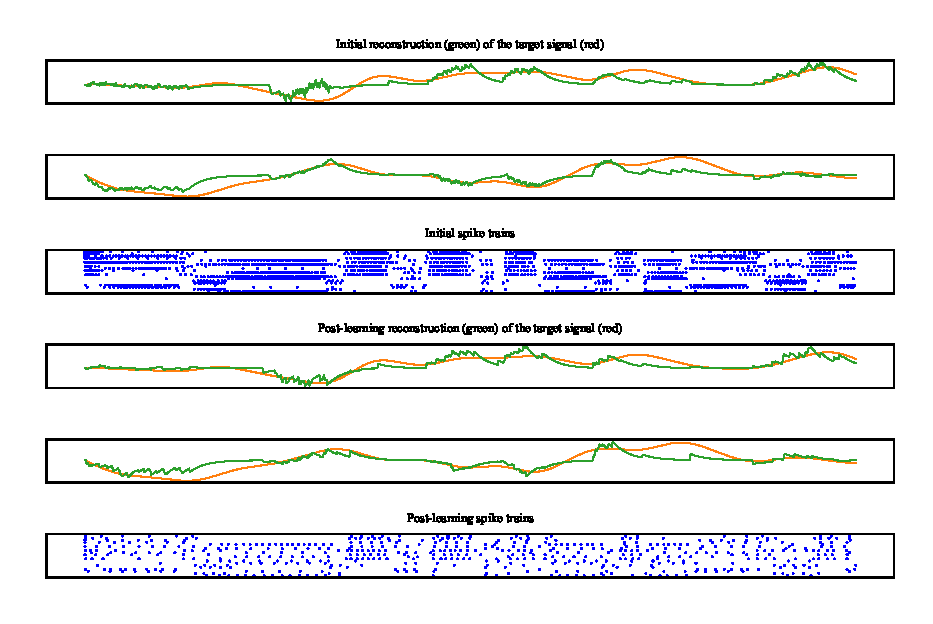
\includegraphics[width = \columnwidth, height=10cm]{figures/DYNAPS_reconstruction.eps}
  \caption{While reducing the reconstruction error, the spike train sparsifies.
  In fact, for this experiment 880 spikes were saved over a period of 1 second, which is more
  than 3 million in one hour. Assuming that a neuron consumes
  $2.468 \cdot 10^ J$, we saved $0.781 J$, only for 20 neurons.}
  %! Correct caption please
  \label{fig:DYNAPS_reconstruction}
\end{figure}

When comparing Figure \ref{fig:DYNAPS_reconstruction} with Figure \ref{fig:reconstruction},
especially the scale of the reconstruction error, it
becomes clear that a lot of precision is lost, due to the simulation-DYNAPS mismatch.
Nevertheless, the results show that this setup successfully learns the optimal recurrent matrix,
reduces the mean firing rate, reduces the decoding error and balances the network
(see Figure \ref{fig:DYNAPS_convergence} for convergence behaviour).

\begin{figure}[!htb]
  \centering
  \includegraphics[width = \columnwidth, height=10cm]{figures/DYNAPS_convergence.eps}
  \caption{Please reproduce figure with correct size!}
  %! Correct caption please
  \label{fig:DYNAPS_convergence}
\end{figure}

\newpage

\section{Discussion}

% Acknowledgements should go at the end, before appendices and references

\acks{We would like to acknowledge support for this project
from the National Science Foundation (NSF grant IIS-9988642)
and the Multidisciplinary Research Program of the Department
of Defense (MURI N00014-00-1-0637). }

% Manual newpage inserted to improve layout of sample file - not
% needed in general before appendices/bibliography.

\newpage

\appendix
\section*{Appendix A.}
%! Show used hyper parameters


\vskip 0.2in
\bibliography{bibliography}

\end{document}